\section{Application Scenarios}
\label{sec:scenarios}
%
We next demonstrate our obstruction-free lens via five use-cases considering scalar density volumes from baggage inspection, 3D flow simulation, radiology, air traffic planning, and diffusion tensor imaging.

\subsection{Baggage inspection: An unusual blunt object}
\label{sec:baggage}
%
In most airports, security agents deal with volumetric data exploration during baggage inspections. While automatic systems are now able to detect densities of harmful substances such as C-4, TNT, and nitroglycerin, and even some prohibited articles such as classical firearms and knives, it remains difficult to identify unusual threats. In addition, baggage inspection faces four main concealment strategies\,\cite{7819413}:

\vspace{0.15cm}
\noindent\textbf{Superposition}: A threat (prohibited object) may be sheltered among dense materials. It is sometimes possible to see through such a `shield' using high penetration (enhanced X-ray power) or image processing (contrast improvement) techniques. However, such techniques are not universally available and also require fine-tuning various parameters, which slows down the inspection process.

\vspace{0.15cm}
\noindent\textbf{Location}: Depending on its location inside the luggage, a threat can be hard to detect. Objects located in the corners, edges, or in the luggage'��s frame are very hard to spot.

\vspace{0.15cm}
\noindent\textbf{Dissociation}: One can conceal a threat by spreading its parts in the luggage, \emph{e.g}, by disassembling a weapon and scattering its parts.

\vspace{0.15cm}
\noindent\textbf{Lure}: A lure can be used to to hide the real threat. For instance, a minor threat like a small scissors can be clearly visible and catch the security agent's attention while a more important threat remains hidden.

Baggage labeled as suspicious either by human inspection or automated scan heuristics need detailed human investigation. Besides physical unpacking, which is time-consuming, one can use `virtual unpacking' tools that segment the 3D scan by a density-based confidence measure and next move the segmented objects away by animation to reduce occlusion\,\cite{Li:2012:LVV:2425296.2425325}. Such systems have been patented and used in production\,\cite{patent}. An important limitation thereof is that, when the automatic segmentation is not optimal, the user needs to manually change its parameters, repeat it, and repeat the animation, which goes back to being time consuming.

Consider the baggage scan in \autoref{f:baggage_lens} with a volume size of 283x189x344 voxels. Automatic baggage inspection systems will not detect anything suspect on this scan. However, while visually exploring this baggage from different angles (\autoref{f:baggage_lens}a-c), it appears that an object is hidden between a set of mugs. A common solution to this type of issue in baggage inspection is to filter materials by density in order to show or hide subsets of the volume and reduce the occlusion. However, in this case, this solution does not work, as the suspect target has almost the same density as the surrounding mugs. Hence, removing the occluders will also remove the target (\autoref{f:baggage_lens}d-f). Using the obstruction-free fish-eye lens helps in this kind of situation. Clicking on the sharp detail visible in \autoref{f:baggage_lens}c first gathers rays so they pass through the low-density zone between the mugs (\autoref{f:baggage_lens}f)

The user has just to use this tool on the partially hidden target. Then, a transition inside the lens will start and smoothly provide the final unobstructed view of the blunt object which is, in this case, a ceramic shuriken (\autoref{f:baggage_lens}e-g). However, this shows only a small part of the target. Scattering rays next fully reveals the target (\autoref{f:baggage_lens}h). The user can adjust the lens size to get a more detailed view of the target (\autoref{f:baggage_lens}i). Next, the user can locally turn the viewpoint around the target, as already shown in \autoref{f:rotation}. From these views, the controller decides that the target is a copy of a shuriken (Japanese ninja star weapon). However, since the object is very thick and blunt (see \autoref{f:rotation}), it is clearly not a threat.

As we obtained this dataset from an airport, we had the opportunity to get feedback on our obstruction-free lens from three baggage security operators. According to them, our tool is interesting as it can provide them a better perception of the items inside the baggage as compared to the classical 2D single-viewpoint X-ray machinery they commonly use. However, this tool should not be used for the typical carry-on baggage inspection where the time-window allowed for inspection is extremely small (about 15 to 20 seconds) in order to keep a smooth traffic flow, for economic reasons. In contrast, this tool is considerably more interesting for inspecting checked-in baggage, where one has a longer inspection time-window (up to 3 minutes). The added value for this use-case is also higher: Opening up checked-in baggage for manual inspection is much more complicated and time-consuming than for carry-on baggage, given its automatic handling. Moreover, the only system for inspecting such baggage currently in use is a scanner that aims to automatically detect suspicious objects in X-ray imagery; this system suffers from false positives, so having a manual in-depth examination tool like our lens can quickly eliminate such false positives, and thus the unnecessary delays they cause when opening up the respective baggage.

\subsection{Fluid flow: A deep-buried spherical vortex}
\label{sec:flow}
%
%
Flow visualization using streamlines has a long history in scientific visualization~\cite{brambilla2012illustrative,merzkirch2012flow}. When applied to 3D datasets, a key challenge is to balance the streamline density. Low values allow seeing inner regions in the data but can subsample (miss) important patterns. High values show more data but create too much occlusion. We next show how our lens can be used to discover interesting patterns in the second case, \emph{i.e.}, a 3D volume densely filled with streamlines. The dataset, introduced in\,\cite{griebel2004flow}, captures the simulation of water flow in a basin computed on a grid of 128x85x42 cells. A set of 4595 streamlines with 183K sample points is next traced by pseudo-random seeding over this vector field. We convert this set of 3D curves (polylines) to a scalar volume by using kernel density estimation (KDE)\,\cite{silverman1986density}. Similar techniques have been used to compute density maps of 2D trail-sets\,\cite{hurter2012graph,cubu,hurter2015image}. To increase computational speed, we compute the KDE in the frequency space and using GPU acceleration, following\,\cite{lhuillier2017ffteb}. The resulting volumes have a resolution of $500^3$ voxels and can be directly displayed using DVR (\autoref{f:stream_lens}). Note that, given the smoothing effect of KDE, streamlines appear now as finite-thickness tubes rather than pixel-thin curves.

For a first overview, we display the volume using standard DVR. After turning the viewpoint a bit, we notice a dense spherical item inside the dataset (\autoref{f:stream_lens}a). To see its shape better, we increase the opacity; however, this immediately increases occlusion so the item becomes invisible. Conversely, decreasing opacity to reduce occlusion makes the item almost transparent. Our lens solves the problem: In the initial view (\autoref{f:stream_lens}a), we point at the target and turn on the lens. This effectively pushes away the occluding stream bundles, and lets us see that our item is nearly perfectly spherical (\autoref{f:stream_lens}b). This is something we could not have assessed from \emph{any} viewpoint and with likely any opacity modulation using standard DVR. Our object is a set of densely-packed, low-speed, tightly-turning streamlines that create a ball-like vortex. Interestingly, this spherical vortex has not been discovered by any of the visualization techniques that we are aware of that used this same dataset\,\cite{telea_vis_99,griebel2004flow,ddh,lhuillier2017ffteb}. To make sure our target is spherical, we view it in the lens from different directions, by interactively changing the ray directions in the lens (\autoref{f:stream_lens}c). Finally, we can close the lens but keep the target magnified (\autoref{f:stream_lens}d).


\begin{figure*}[htb]
\centering
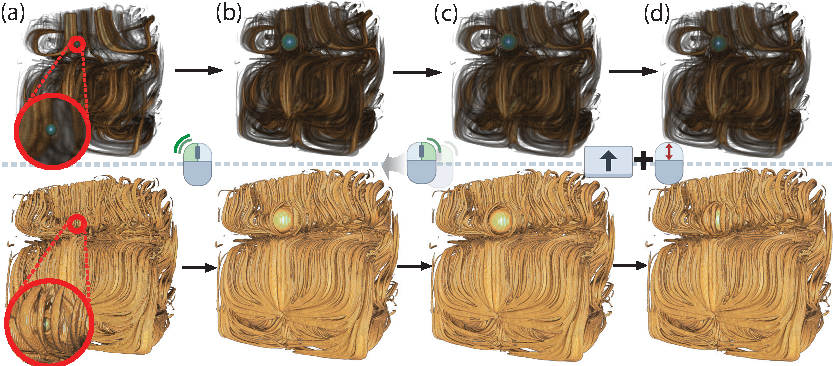
\includegraphics [width=0.95\textwidth]{images/stream_lens.eps}
\vspace{-0.15cm}
\caption{Flow volume exploration with two different opacity transfer functions (top and bottom rows). In viewpoint (a), we notice a small high-density spherical item. (b) We apply the lens at that location (double click). (c) The directions of rays in the lens are changed to see the whole target in the lens (right click + mouse drag change direction). (d) The lens is gradually closed while keeping the focus area magnified (shift + scroll).}
\vspace{-0.15cm}
\label{f:stream_lens}
\end{figure*}

\subsection{Chest scan: A hard to see tumor}
\label{sec:chest}
%
In our third use-case, we consider a contrast chest CT scan (512x512x110 voxels) of an elderly patient having a sizeable lung tumor. The tumor was detected at a CT scan ordered by the pulmonologist in charge of the patient, after the patient reported acute chest pain. Typical examination of these scans by the pulmonologist and radiologist in charge involves slice-based views. Figures~\ref{f:slicer}a-c and \ref{f:slicer}d-f show two such slice sets (axial, coronal, and saggital views), produced using typical lung, respectively mediastinal, contrast presets. Although the tumor is visible in all these views, its exact shape, morphology, and connection to the lung walls are not easy to assess. Finding such details on the tumor is essential, explained both doctors in charge, for determining the TNM score and also planning treatment. Using standard DVR makes the tumor and its 3D position partially visible (\autoref{f:slicer}f). However, occlusion from the rib cage and other tissues is still present. Using both TF presets and manually changing the TFs in the 3D Slicer tool\,\cite{slicer} used to create the DVR could not help de-occluding the tumor without making (parts of) it transparent. This is also visible in the slice images in \autoref{f:slicer}a-f, where the gray values for the tumor and surrounding skin-and-muscle tissue on the rib cage are very similar. 
This density similarity is due to the fact that the tumor had grown rapidly in a short time span, explained the pulmonologist. As such, the tumor started necrotizing, which filled it with fluids, making its density very similar to that of the obstructing (skin and muscle) tissue. In conclusion, one cannot remove such occluding tissue in a classical DVR setting by opacity TF manipulation without also removing the tumor. This situation makes examining this specific tumor harder than for regular cases.

\begin{figure}[htb]
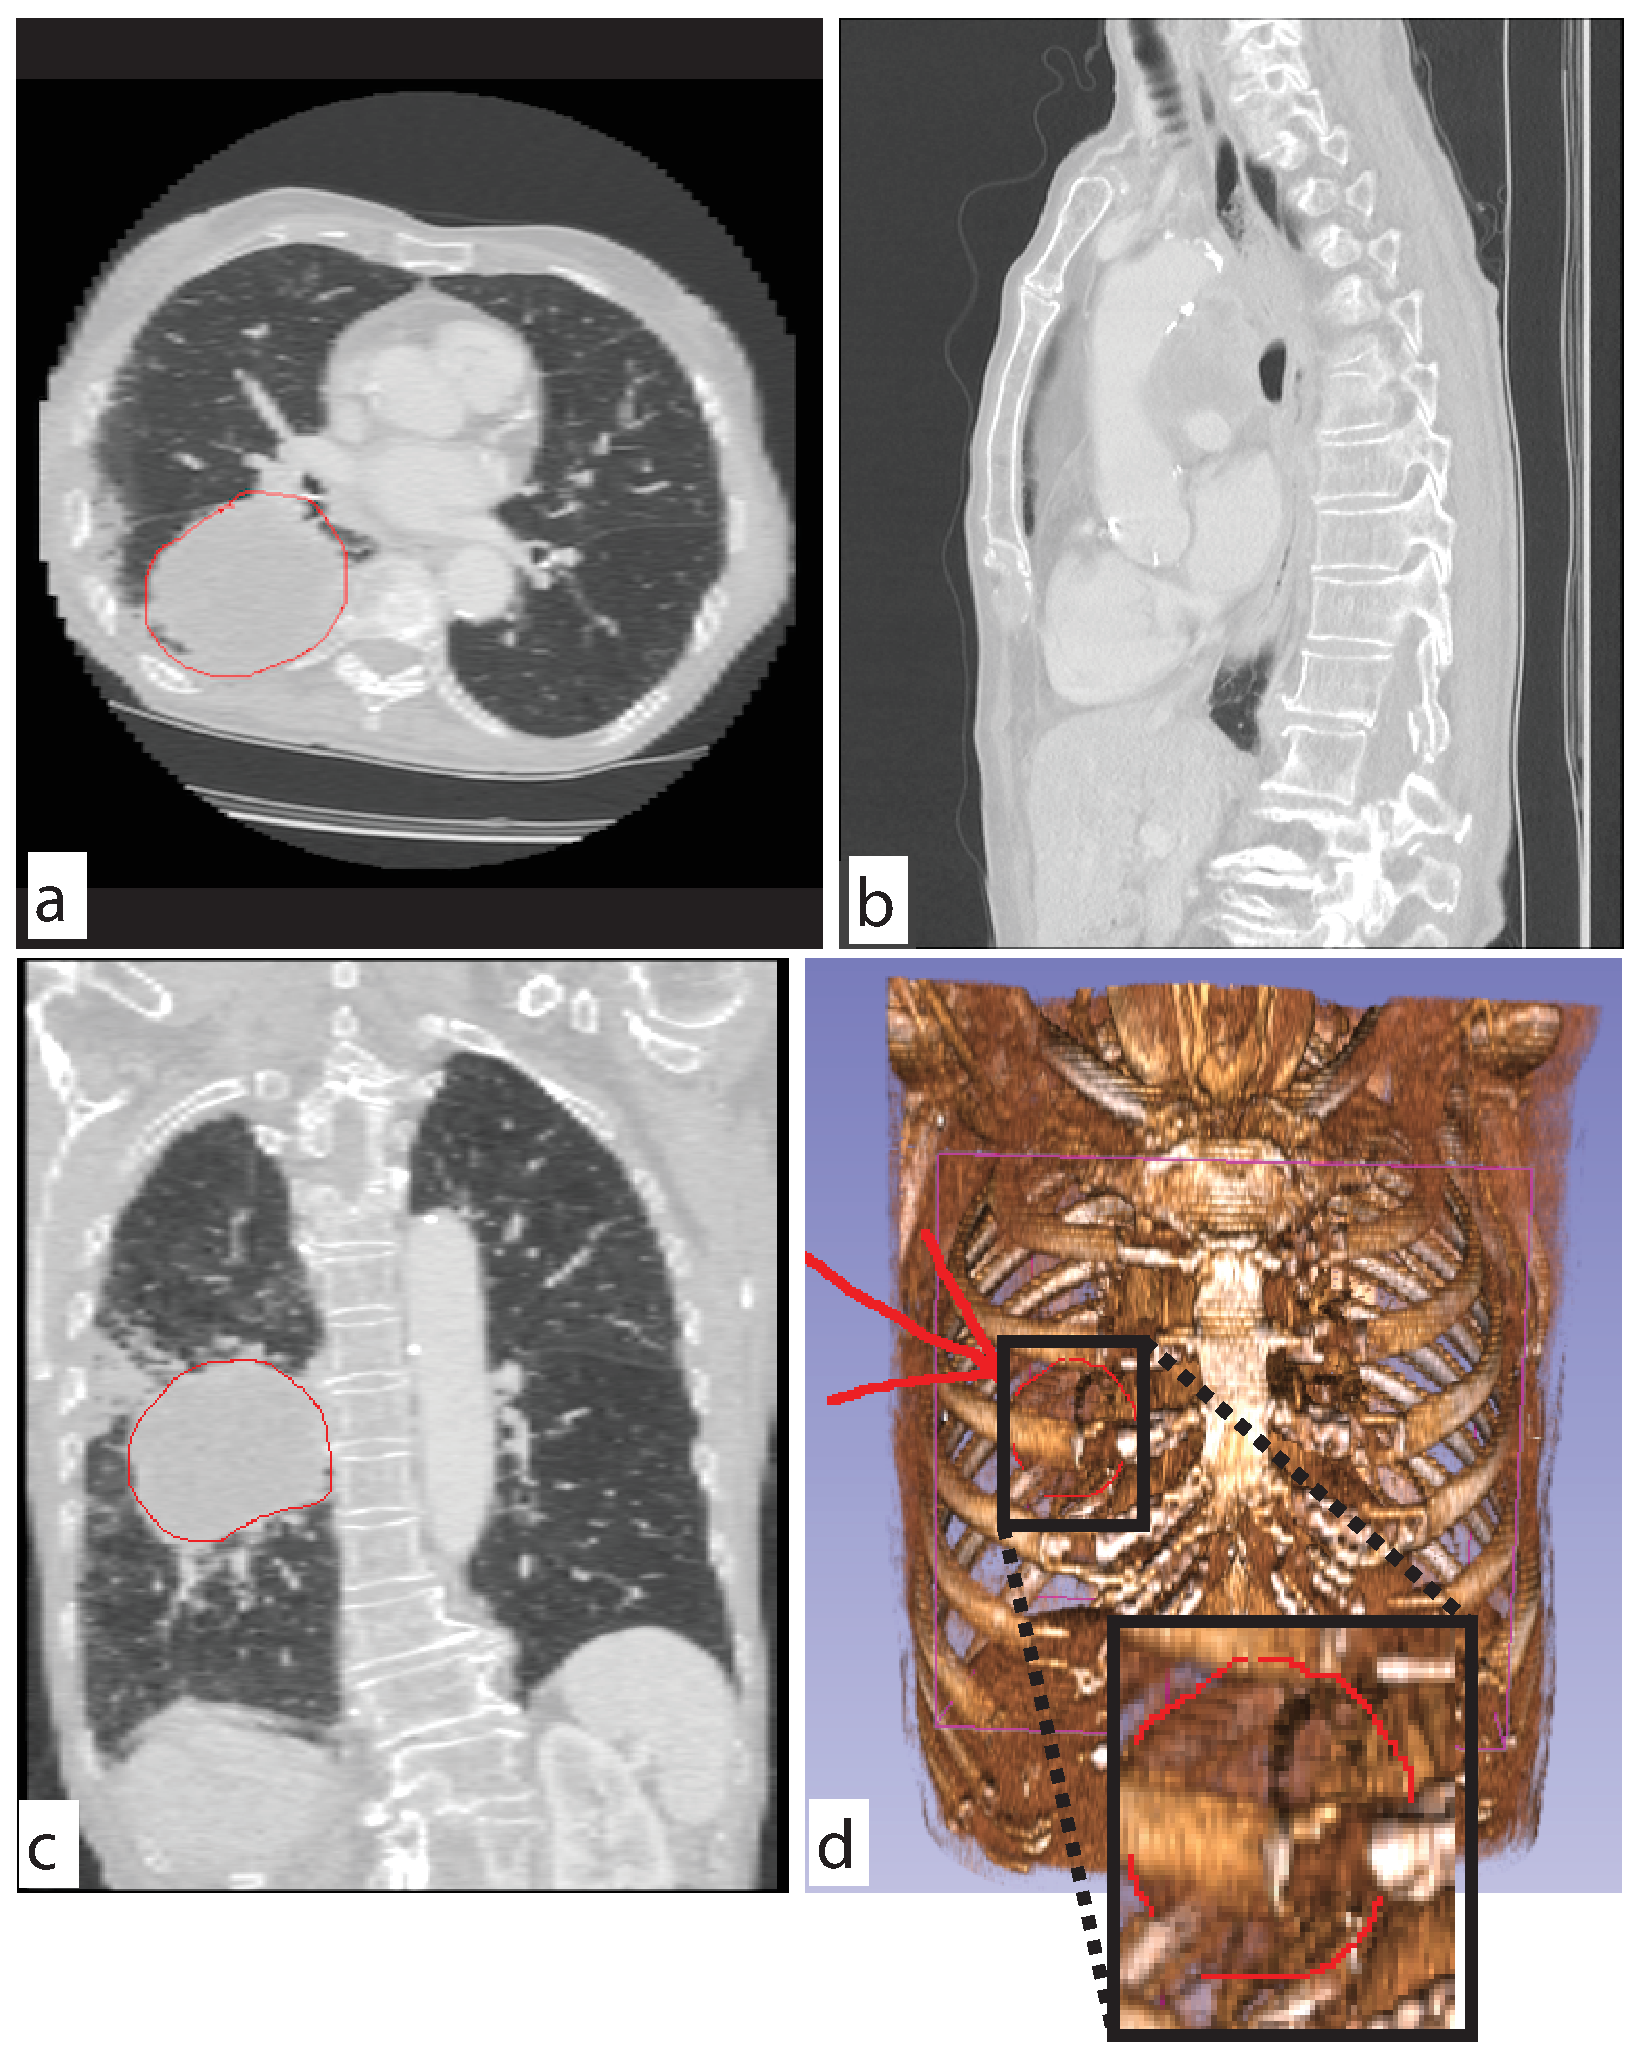
\includegraphics [width=0.48\textwidth]{images/slicer.eps}
\caption{Lung tumor visualization using slices (a-c) and standard DVR (d). Annotations are manually added by the examiner to delineate the tumor location. Images constructed using the 3D Slicer tool\,\cite{slicer}.}
\label{f:slicer}
\end{figure}

We next used our lens to examine the tumor. Sample snapshots obtained in this process are shown in \autoref{f:params}. Comparing these with standard DVR (\autoref{f:slicer}d), several points can be made. First, the tumor is significantly more visible when using the lens, both in terms of removing the occluding tissue and in terms of the tumor's opacity -- compare the inset in \autoref{f:slicer}d with the images in \autoref{f:params}. Secondly, relighting the tumor from various directions allows one to see small-scale morphological details such as the tumor's surface shape and its connection via protuberances and veins with the lung walls.

To assess the added-value of our lens, we asked the two medical specialists (pulmonologist and radiologist) involved in treating the patient that this dataset came from to study the lens' features and state its potential advantages and/or limitations as compared to standard slicing and DVR techniques they use in their practice. Both specialists have over 10 years of medical experience in treating lung cancer, and routinely use several slicing and DVR software tools. They work in a private hospital in Belgium and are not actively associated to medical imaging research. Moreover, our (authors') identities were hidden from them, by using a third person in the communication. The provided input can be summarized as follows: The occlusion-free lens is definitely easier and faster to use than classical DVR and/or slicing techniques. It is especially more effective than these to get a quick, first impression of a deep buried anatomical detail. Changing the lens' parameters by direct interaction is as simple as changing window/level functions in a typical slice-based visualization, and is definitely simpler than tuning typical DVR parameters to obtain similar results. This `entices' the user to explore, which is a good aspect. The fact that the lens minimizes viewpoint change (volume rotation), \emph{i.e.}, after a suitable viewpoint was found from which a (small) part of the target is visible, one doesn't need to change this viewpoint, is a strong feature, as 3D viewpoint changes are disruptive and cost time. This is important in a cost-aware environment where specialists have very limited time (10-15 minutes) to  assess a CT scan. However, the lens cannot and should not replace classical slice-based investigation, which shows small-scale details better. This is especially important when examining small-size lesions, tumors, or other similar anatomical features, that the lens will arguably not be able to help with, as these are too small in the first place to attract the attention of the examiner looking at a standard DVR rendering. In the context of the current dataset (Fig.~\ref{f:slicer}), the lens was useful to both confirm the TNM score (T3 grade tumor, 6.5 cm in size) found via the 2D slices, but much more so for inderstanding how and where the tumor is connected to surrounding tissue, which is very hard to do using only 2D slices.

\begin{figure}
\centering
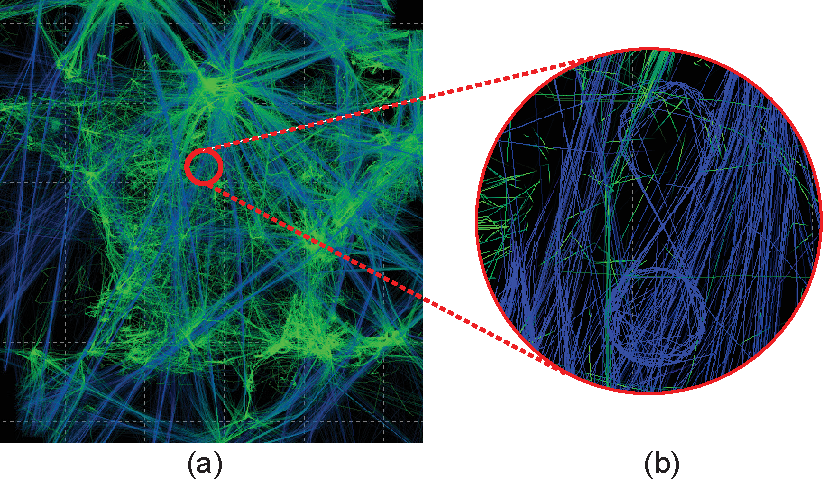
\includegraphics [width=0.48\textwidth]{images/aircraft.pdf}
\vspace{-0.15cm}
\caption{Visualizing one day of aircraft trajectories over France\,\cite{hurter2009fromdady}. (a) Overview of all trails. (b) Zoom, filtering, and color mapping techniques are used to highlight an outlier trajectory of an aircraft performing an eight-shaped loop. Revealing this outlier costs significant user effort.}
\label{f:fromdady}
\vspace{-0.15cm}
\end{figure}


\subsection{Aircraft trajectories: Outliers in the French sky}
\label{sec:atc}
%
%
We next consider a task from the air traffic planning field -- detecting and studying outliers in large-scale datasets containing tens of thousands of 3D (latitude, longitude, height) trails of aircraft over a given spatio-temporal region\,\cite{hurter2014interactive}. Typically, such datasets are displayed using 2D (latitude, longitude) plots where opacity encodes the spatial density of flights. \autoref{f:fromdady}-a shows one day of recorded aircraft trajectories over the French air space using this 2D technique. \autoref{f:fromdady}(b) shows a detail zoom-in of this dataset, where we can see an abnormal -- that is, far from straight or slightly curved -- aircraft trajectory: A tanker aircraft performed an eight-shaped loop as it was waiting to refuel other aircraft. Revealing such patterns using 2D techniques, \emph{e.g.} \cite{hurter2009fromdady}, is very hard. In particular, it is hard to de-occlude these patterns from the overall context of criss-crossing aircraft trails, even when one knows their 2D spatial location.

Our lens can help for this task, as follows. We first convert the set of 3D trails to a $500^3$ density volume, using KDE as described for the streamline use-case (Sec.~\ref{sec:flow}). Examining this volume using standard DVR allows us to see that there is an outliner (that is, not straight) trail at some point in space, see curved patterns in \autoref{f:aircraft_lens}a. By activating the lens on this area and interactively tuning the target depth $t_{min}$ (since we don't know the height of this trail), we can quickly obtain a view where the outlier trajectory is in focus and the occluding ones are pushed away (\autoref{f:aircraft_lens}a). Finally, just as in the other examples presented so far, the user can quickly change the magnification factor and view direction to better study this trajectory in context (\autoref{f:aircraft_lens}b-d). From these images, one directly and easily sees that the outlier trajectory has an eight shape. Revealing this outlier trail using standard 2D visualization techniques\,\cite{hurter2009fromdady} costs several minutes. Doing the same using our lens approach costs under one minute, for the same users. Additionally, if we compare Figs.~\ref{f:fromdady}b and~\ref{f:aircraft_lens}b-d, we argue that the eight-shape of the outlier trajectory is much more prominent, and thus recognizable, in the latter images (using our lens) than in the former ones. Last but definitely not least: The 3D volume rendering approach that our lens is based on explicitly encodes the flight height information, so our lens can use it by interactively tuning the depth value $t_{min}$ where the lens is focused. This is not possible with 2D techniques which ignore this depth dimension.

We validated our findings with an air traffic data scientist with more than 10 year experience in air traffic control and air traffic planing. She confirmed that this specific eight-shape trail in \autoref{f:fromdady}(b) is an actual aircraft which performed waiting loops and acted as a fuel supplier for military aircraft. Other comments included the following: Compared to standard 2D visualization techniques, our tool makes detecting outliers easy since there is no need for complex manipulation to reveal such outlier trails. Also, the user does not have to deal with color and alpha mapping parameter-tuning to make specific outliers emerge. Separately, trail visualization easily creates many occlusions leading to either fully opaque areas or too much local overlap, both which hinder seeing and examining specific trails. Our lens does help such cases by distorting the space to locally remove such occlusions. All in all, in the studied dataset (\autoref{f:fromdady}), the lens was specifically useful since, for high transparency, one would not detect the outlier trail, while for low transparency, one would get a hint of the outlier's existence, but not see it in detail due to too much occlusion; the lens allows using low transparency, but removes the clutter caused by it to reveal the outlier.


\begin{figure*}[htbp]
\includegraphics [width=0.98\textwidth]{images/aircraft_lens.pdf}
\caption{Inspecting an abnormal aircraft trail. (a) The abnormal trail is spotted in an all-trails view as it is highly curved while all other trails are relatively straight. Activating the lens at the outlier location (b) and changing the magnification factor (c) reveals the trail's eight-shape. (d) Rotating the viewpoint provides spatial insight on the embedding of the outlier in the surrounding trails.}
\label{f:aircraft_lens}
\end{figure*}
%

\subsection{Brain fibers: Uncluttering the bridge}
\label{sec:dti}
%
Finally, we consider a last example related to the exploration of fiber tracts visualized as streamlines of the major eigenvector of a diffusion tensor imaging (DTI) field. Such datasets shows a spatially complex structure which makes them hard to explore\,\cite{assaf08}. In particular, fiber tracts are spread volumetrically over the entire extent of the brain, and create tangled patterns which make it very hard to see deep within the emerging structures. DVR techniques are often used to render such fiber tracts, one of the advantages being that close fibers get visually `merged' to reveal spatially coherent structures, an effect which is not possible when fibers are rendered using polyline (streamline-like) representations. However, DVR methods also create more occlusion, thus difficulties in seeing structures deep within the volume.

For this use-case, we use an $128\times128\times51$ DTI volume ( same dataset as in~\cite{everts15}). From this volume, we traced 150352 fibers seeded in, and going over, regions of high fractional anisotropy. Next, we filtered out fibers shorter than 2mm, yielding a total of 120593 fibers to display (6.4M sample points). Next, we converted this fiber-set to a $512^3$ density volume, using kernel density estimation with a 3D isotropic kernel of radius 15 pixels. The conversion process is identical to the one used for the streamlines in Sec.~\ref{sec:flow}. Figure~\ref{fig:dti}a shows the result, rendered with DVR, with a simple opacity function mapping the fiber density. While terminal fibers are well visible, it is impossible to discern anything inside the volume. Activating the lens in the middle of the volume opens a hole through which a small part of the \emph{corpus callosum}, the fiber bundle wrapping the bridge that connects the two emispheres, becomes visible. To obtain an even better view hereof, we slightly decrease the opacity (Fig.~\ref{fig:dti}c). The \emph{corpus callosum} is now clearly visible, appearing as a compact structure, due to the KDE blending of neighbor fibers. Note that obtaining such a view on the \emph{corpus callosum} using only DVR would be very hard, since transfer functions would either render separated (non-merged) fibers, or else make the fibers surrounding the structure of interest too thick and occluding. 

There is one notable difference to this scenario as compared to all previous ones. In all earlier cases, the standard DVR of the data (that is, without the activated lens) showed us a partial small cue of the structure of interest within the volume, and we used the screen-space location of this structure as the center point where to activate the lens. In this last scenario, there is no clear point within the original DVR image (Fig.~\ref{fig:dti}a) from which the \emph{corpus callosum} is even partially visible, due to the high opacity given by the transfer function used. As such, the user activates the lens here at \emph{any} desired point to peek inside, and towards the center of, the volume. However, given the nature of the data, the structure of interest is quite easily visible from most such viewpoints (see lens inset in Fig.~\ref{fig:dti}b). Once its presence is revealed, the user can next adjust the viewpoint and/or the opacity transfer function to get an optimal view on the target, such as the one shown in Fig.~\ref{fig:dti}c.

\begin{figure}[htbp!]
\centering
\includegraphics [width=0.45\textwidth]{images/dti.eps}
\caption{Revealing the \emph{corpus callosum} in a DVR of a set of DTI tracts.}
\label{fig:dti}
\end{figure}


%
